\section{进程管理}
在正式介绍Linux内核中的进程和线程前,
我们先利用课程中了解到的进程和线程的概念尝试直接分析内核中进程的表示方式——进程控制块(PCB),
建立整体的认识.
最后,我们试着弄懂Linux的进程调度策略,并把重点放在最常用的
Completely Fair Scheduler(CFS)上.

\subsection{进程控制块}
\lstinline{struct task_struct}\index{t@\lstinline{task_struct}|alsoname {PCB}}
是Linux内核的进程控制块(PCB)\index{PCB}.
它存储进程的标识符、进程的状态、指向存储进程上下文的数据结构的指针、调度所需的信息以及与进程相关的资源和指向其他 \lstinline{task_struct} 的指针等.
所有与进程有关的操作都会直接或间接地修改进程控制块来达到目的.
下面,我们介绍管理进程所需要的多种信息,并介绍它们是如何在 \lstinline{task_struct} 中表示的.

\begin{readsrcbox}{进程控制块}
	\lstinline{struct task_struct} 是在\linuxsrc{include/linux/sched.h}中定义的.
\end{readsrcbox}

\subsubsection{进程的状态} \label{process state}
首先是进程的状态,一个进程可能处于这些状态\index{process state}:
\begin{itemize}
	\item \lstinline{TASK_NEW}.
	      当一个进程刚创建时,它的状态就被设置为\lstinline{TASK_NEW},表示这个进程已经被创建,但是还没有开始运行.
	\item \lstinline{TASK_DEAD}.
	      进程已经结束.
	\item \lstinline{TASK_RUNNING}.
	      进程正在运行,即该进程在正在运行的进程的队列里.
	\item \lstinline{TASK_INTERRUPTIBLE} 或者 \lstinline{TASK_UNINTERRUPTIBLE}.
	      处于这两个状态的进程正在等待,但是只有 \lstinline{TASK_INTERRUPTIBLE} 状态的进程才会被信号唤醒.
	\item \lstinline{TASK_NOLOAD}.
	      类似 \lstinline{TASK_UNINTERUPTIBLE} 但是在统计数据中不被计入负载.
	      \footnote{见 \url{https://lore.kernel.org/lkml/alpine.LFD.2.11.1505112154420.1749@ja.home.ssi.bg/T/}}
	\item \lstinline{TASK_WAKING}.
	      进程已经被要求唤醒,但是还没有进入正在运行的进程队列.
	      \footnote{见 \url{https://lore.kernel.org/lkml/tip-e9c8431185d6c406887190519f6dbdd112641686@git.kernel.org/}}
	\item \lstinline{TASK_WAKEKILL}.
	      该进程收到SIGKILL信号时会被唤醒.
	\item \lstinline{TASK_TRACED}.
	      调试器暂停该进程来追踪它的运行状态.
\end{itemize}
这些状态被编码成掩码,读写进程的状态时,
需要用这些掩码操作 \lstinline{task_struct} 的 \lstinline{__state} 域.
比如识别一个进程是否处于某状态,
就要用它的 \lstinline{__state} 和 这个状态的掩码做与操作,
若结果为0则不处于这个状态.
这些状态中有的状态可以组合成新的掩码,方便使用.

\subsubsection{进程的CPU上下文} \label{context}
进程控制块还需要存储有关进程上下文的信息,例如有关栈和堆的信息和CPU内部寄存器的值.%
\index{process context}
这一部分信息既和内核的内存管理有关又依赖于具体的硬件架构,
是实现进程调度中挂起和重启进程所需要的数据结构.
\begin{readsrcbox}{架构相关代码}
	为了提高可移植性,Linux内核的代码区分不依赖于具体硬件架构的代码和针对特定架构的代码.
	架构相关的代码全部在 \linuxsrc{arch} 目录下.
	例如 x86和x86\_64的代码位于 \linuxsrc{arch/x86}.

	显然,所有的汇编代码都应该放在该目录.
	内存管理和进程管理所需的某些功能也依赖于CPU的特定功能,
	需要根据硬件功能定义数据结构和执行具体的指令,
	这些定义和实现也位于 \linuxsrc{arch} 下具体架构的目录下.
	不同的架构的代码尽量暴露出相同的接口,供架构无关代码使用.

	某一架构上的具体实现的文档可以在 \href{https://docs.kernel.org/arch.html}{\lstinline{Document/arch.rst}} 中的列表找到.
	例如\href{https://docs.kernel.org/x86/kernel-stacks.html}{\lstinline{Document/x86/kernel-stacks.rst}}介绍了x86\_64 CPU上内核为每一个进程维护的若干个栈.
\end{readsrcbox}
\lstinline{task_struct}的定义中,有一个 \lstinline{void *stack;} 域.
这不是该进程的用户态的栈的起始地址,
而是该进程的\textbf{内核栈}的起始地址,每次该进程通过系统调用从用户态进入内核态时,
内核中的代码都在这个内核栈上执行.\index{kernel stack}

\lstinline{tast_struct}的最后一个成员是 \lstinline{struct thread_struct thread;}%
\index{t@\lstinline{thread_struct}},
进程在CPU上的运行状态存放在这个架构相关的结构体中.
x86\_64上该结构体的大小可以变化,因此它必须作为\lstinline{tast_struct}的最后一个成员.
这个 \lstinline{struct thread_struct} 的成员直接或间接地保存该进程的上下文.

我们在微机原理中学过x86\_32架构对于上下文切换有专门的硬件支持.
Global Descriptor Table(GDT)中有专门的描述符指向Task State Segment(TSS)%
\index{TSS}.
TSS可以用来存储所有的x86寄存器,
在需要时自动进行硬件上下文切换,把寄存器的值存储在旧的TSS中,然后把新TSS的内容加载到寄存器中.
x86\_64取消了硬件上下文切换的功能,但即使是在32位x86机器上,
Linux内核也不是用TSS来进行硬件切换,
因为考虑到其它架构几乎都不支持这一机制,使用软件实现上下文切换可移植性更好.

Linux 内核在上下文切换时,寄存器的值实际上是存在进程的内核栈上的.
进程在切换之前,一定正在该进程的内核栈上执行内核态的代码,
这时用户程序的寄存器已经在进入内核态后保存下来了,
要保存运行在内核态时的寄存器,只需要 \lstinline{pushq} 所有的\textit{被调用者保存}寄存器即可.
这是因为在进入当前栈帧前后,调用者一定已经保存了其所需的\textit{调用者保存}寄存器.
返回地址也在栈帧中有记录.
既然这个栈帧就记录着当前进程的上下文,PCB只需保存这个栈帧的地址即可.
因此 \lstinline{thread_struct} 有一个 \lstinline{unsigned long sp;} 域,
存放的就是切换前的寄存器sp的值,即这个栈帧的地址.

除了整数运算的寄存器,浮点和向量运算的寄存器也需要保存,
但是由于浮点和向量运算不像整数运算那样常见,
且保存这些状态有一定开销,
之前的Linux内核只在这些运算真正执行过时才保存对应的寄存器.
这种“懒惰”的保存方式是通过CPU的硬件支持完成的:
每次上下文切换时,CPU的TS标志位就被置为1;
每次浮点或向量运算指令执行时,若TS标志位为1,则会报“Device Not Available”异常.
内核在处理这个异常时会记录下来:该进程使用了浮点或向量运算.
再次切换进程时,若发现使用了浮点或向量运算,则保存相应的状态.\cite{bovet2005understanding}
而现代的CPU引入了特定的指令来保存FPU状态,
减小了保存FPU状态的开销,
而且程序越来越依赖向量指令来进行拷贝数据等操作,
所以Linux在2016年取消了“懒惰”的保存方式,
\footnote{见 \url{https://lore.kernel.org/lkml/e3b2baadcd19bf8abcd3bcd60d19e8e50e75f63a.1453510332.git.luto@kernel.org/}}
每次进程切换都保存FPU的状态.
除了进程切换,
另外一个需要保存和恢复FPU状态的时机是内核代码在用户上下文中使用浮点或向量运算的前后,
这也是按需进行的,
即返回用户态时,若改变了FPU状态才加载用户的FPU状态.

FPU的状态保存在 \lstinline{thread_struct} 的 \lstinline{struct fpu fpu;}域.
这个数据结构是变长的,这也是 \lstinline{struct thread_struct thread;}
要放在 \lstinline{task_struct} 最后的原因.

\begin{readsrcbox}{\lstinline{thread_struct}}
	\lstinline{thread_struct}\index{t@\lstinline{thread_struct}} 是架构相关的.
	x86的 \lstinline{thread_struct} 的定义在 \linuxsrc{arch/x86/include/asm/processor.h} 中.

	进程调度总是通过调用一个名为 \lstinline{schedule()}\index{s@\lstinline{schedule()}}
	(\linuxsrc{kernel/sched/core.c}) 的函数来实现.
	真正完成调度的函数为 \lstinline{__schedule()}(在同一个文件),
	其上方的注释说明了所有会调用它的情况.

	而最终完成进程切换的是一个名为 \lstinline{switch_to(prev, next, last)} 的宏
	\footnote{x86上的定义在 \lstinline{arch/x86/include/asm/switch_to.h}.
		64位机器的实现,汇编部分在 \lstinline{arch/x86/entry/entry_64.S};
		C语言部分在 \lstinline{arch/x86/kernel/process_64.c}}.
	其关键的操作就是切换进程的内核栈(见图~\ref{fig:switch_to}):
	\begin{enumerate}
		\item 将被调用者保存寄存器压入栈;
		\item 把rsp寄存器存入原来进程的 \lstinline{thread->sp};
		\item 把新进程的 \lstinline{thread->sp} 放入rsp寄存器;
		\item 最后从新的栈中弹出所有调用者保存寄存器.
	\end{enumerate}
\end{readsrcbox}

\begin{figure}[]
	\centering
	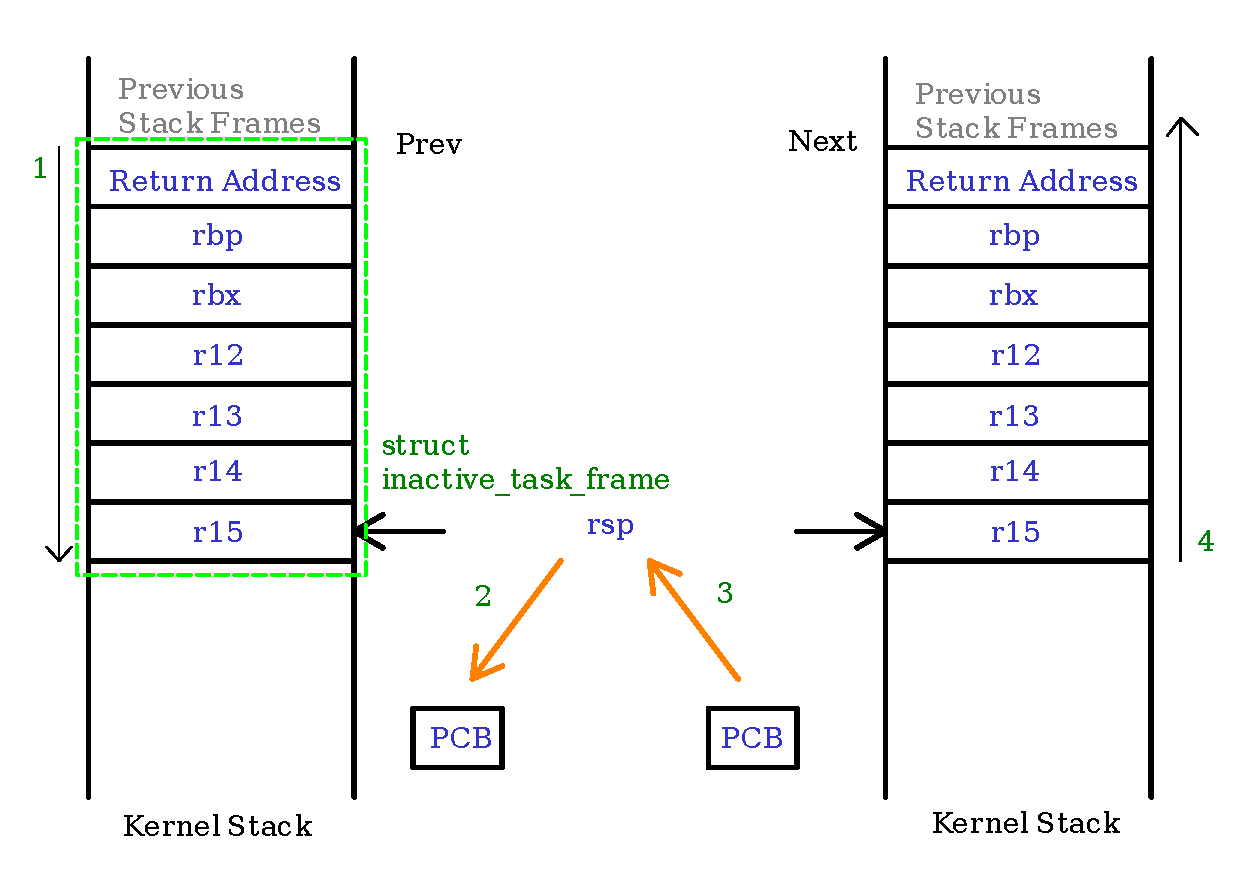
\includegraphics[width=\textwidth]{img/switch_to.pdf}
	\caption{\label{fig:switch_to} 进程切换中的内核栈切换}
\end{figure}


\begin{qbox}{\lstinline{struct thread_info} 与 PCB是什么关系呢?}
	\lstinline{struct task_struct}是进程控制块,
	而 \lstinline{struct thread_info}\index{t@\lstinline{thread_info}}
	存放的也是进程信息,
	只是这些信息更接近底层硬件,且需要能在汇编代码中直接使用.
	\lstinline{struct thread_info} 的大小被控制在一个cache行内,这是由于这些底层信息需要被频繁查看,cache miss会造成较大影响.
	为了尽量利用空间,所有信息都按位编码在其中.
	例如,上文提到的“内核使用了浮点或向量运算而需要加载原来的FPU状态”,
	就存储在 \lstinline{thread_info} 的第 \lstinline{TIF_NEED_FPU_LOAD}
	\footnote{\lstinline{arch/x86/include/asm/thread_info.h} 中定义的宏.} 位.

	\lstinline{struct thread_info} 在更早的Linux版本中位于进程的内核栈的起始位置
	\cite{bovet2005understanding},
	可能造成一些疑惑.
	现在的x86 Linux内核默认把 \lstinline{struct thread_info} 放入
	\lstinline{struct task_struct},
	与PCB的其他成员处于类似的地位.
	\footnote{见 \url{https://lore.kernel.org/all/cover.1473801993.git.luto@kernel.org/}}
	\footnote{见 \url{https://lore.kernel.org/all/a50eab40abeaec9cb9a9e3cbdeafd32190206654.1473801993.git.luto@kernel.org}}
\end{qbox}

\subsection{标识符、进程控制块的链表} \label{process identifiers}
识别进程的方式有很多,首先,指向\lstinline{task_struct} 的指针就可以唯一地确定一个进程.
每一个进程还有编号,记录在 \lstinline{pid_t pid;} 域中.\index{PID}
每一个进程按照创建顺序编号,每一个进程的这个 \lstinline{pid} 域都不相同.
由于 \ref{creating task} 中会介绍的原因,
操作系统的使用者会期望某些调度单元的PID相同.
这是通过 \lstinline{task_struct} 的 \lstinline{pid_t tgid} (thread group id) 域来实现的.
不同的 \lstinline{task_struct} 的 \lstinline{pid} 不能相同,
\lstinline{tgid} 却可能相同.
用户所得到的PID实际上是 \lstinline{task_struct} 中的 \lstinline{tgid} \index{t@\lstinline{tgid}}
而不是 \lstinline{pid}.

进程的产生和销毁是动态的,这意味着进程控制块也需要动态分配,
所有分配出来的进程控制块的地址都要通过某种方式留存起来,以供访问.
Linux内核记录多个进程控制块的方式之一是建立包含进程控制块的双向链表.
链表有多种实现,节点互相链接,每个节点指向一个表内的实体的方式为“非侵入式(non-intrusive)”的链表,
实体中包含所需的链表指针的链表为“侵入式”链表.\index{intrusive linked-list}
如果比较访问下一个节点数据的性能,非侵入式链表比侵入式链表性能更好,
因为非侵入式的链表少一次解引用的访存操作.
另外,寻找链表首尾元素和双向遍历的功能也比较重要,
因此内核使用的链表是侵入式的双向链表.

如图~\ref{fig:task_list}所示,
\lstinline{struct list_head} 作为链表的节点,\index{l@\lstinline{list_head}}
有 \lstinline{prev} 和 \lstinline{next} 两个指针,
分别指向前一个节点和后一个节点.
链表中的元素通过成员中的 \lstinline{struct list_head} 就可以互相链接.

除了构成全系统的进程表的 \lstinline{struct list_head tasks},\index{task list}
\lstinline{task_struct} 中还包括其他的 \lstinline{list_head},
用于记录与该进程相关的其他进程.
比如,记录树形的父子进程的关系(见\ref{creating task}),
就是通过 \lstinline{struct list_head children}
和 \lstinline{struct list_head sibling}这两个链表实现的.
显然,类似于树的Leftmost child, right sibling表示法\cite{sedgewick2001algorithms},
\lstinline{children} 指向的就应该是某个子进程的 \lstinline{sibling} 成员,
而不是 \lstinline{children} 成员.
以创建进程为例,需要把当前进程的 \lstinline{sibling} 成员,
插入到父进程的 \lstinline{children} 所指的链表尾部:
\begin{lstlisting}[language=C]
/*
 * kernel/fork.c
 * copy_process()
 */
list_add_tail(&p->sibling, &p->real_parent->children);
\end{lstlisting}
\begin{figure}[]
	\centering
	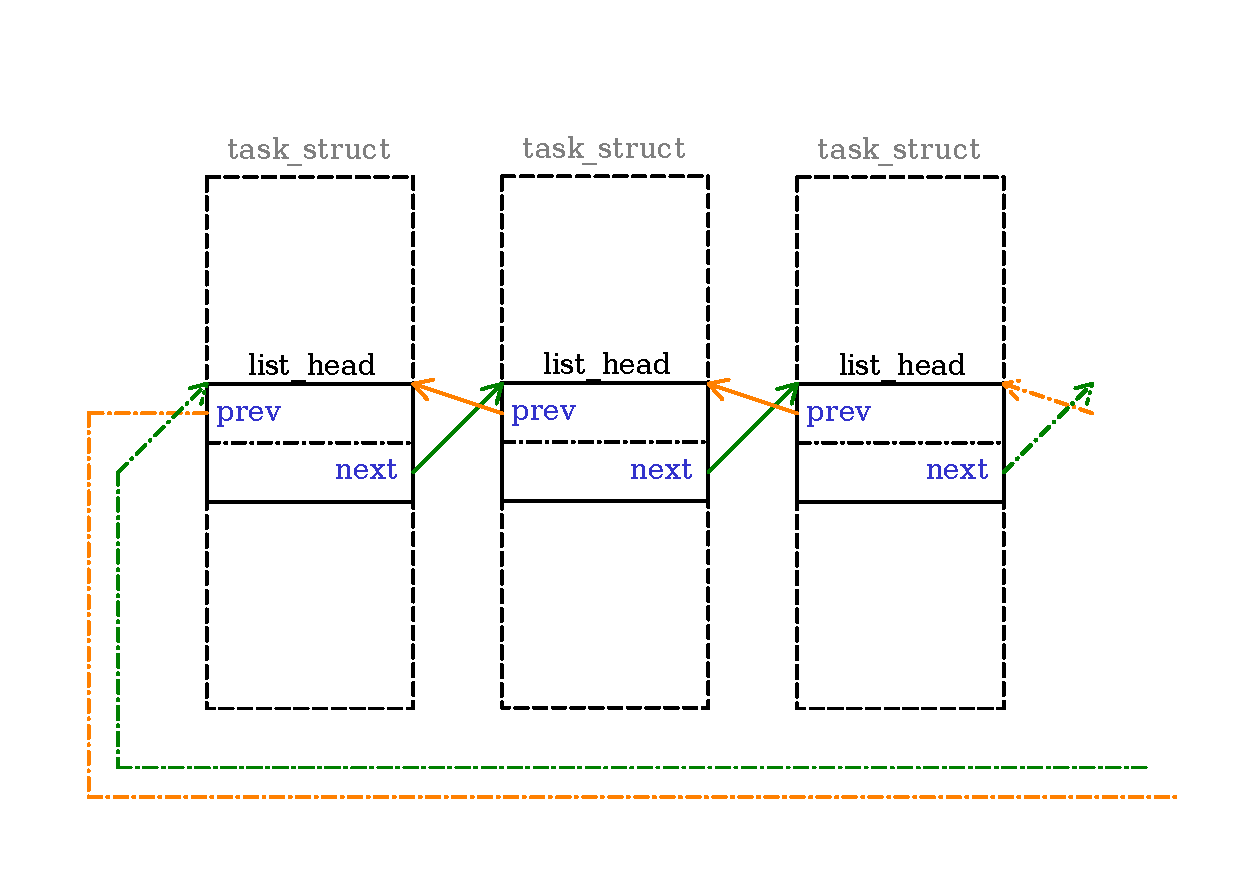
\includegraphics[width=\textwidth]{img/intrusive_list.pdf}
	\caption{\label{fig:task_list} 侵入式双向链表}
\end{figure}

进程控制块还需要通过PID快速获取,这是通过散列表实现的,这里不详细介绍.

\subsubsection{其他信息}
进程控制块中还包括这些方面的相关信息:内存管理、打开的文件、文件系统、调度器、统计数据等.

\begin{itemize}
	\item\textit{内存管理:} 进程的虚拟地址空间信息,\textbf{页表}(将在 TODO 中介绍)
	\item \textit{文件:} 内核需要维护进程\textbf{打开的文件的表},以记录该进程读写文件的状态.
	\item \textit{文件系统:} 记录进程的\textbf{工作目录}和,操作文件所用的\textbf{权限}等.
	\item \textit{调度:}进程所属的\textbf{调度类型},进程的\textbf{优先级}等.
	      (将在\ref{scheduling}中介绍)
	\item \textit{异常处理/进程通信:}进程等待接收的\textbf{信号},信号的屏蔽情况,\textbf{信号处理程序}的地址.
\end{itemize}

\subsubsection{进程和线程的创建} \label{creating task}

\begin{qbox}{内核中线程和进程的区别是什么?}
	前文我们一直以“进程”来描述Linux内核调度的单位.
	即使代码中出现了 \lstinline{thread} 的字样,
	我们仍用“进程”指代.
	实际上,Linux一直使用task来称呼调度的单位,
	只是在和CPU线程有关的地方使用了thread的说法.
	下文将涉及Linux内核中线程和进程的区别.
\end{qbox}

内核中第一个进程是在启动时创建的,PID为0,名为空闲进程(the idle thread),
内核中有一个 \lstinline{struct task_struct init_task}
作为静态的全局变量,在启动时各个成员被赋上相对固定的初始值.
在内核的启动过程中,空闲进程进行一定的初始化,
然后就创建PID为1的进程(the \lstinline{init} process)%
\index{i@\lstinline{init}},
进一步初始化,最后载入init程序\cite{bovet2005understanding}
(Arch Linux中即为systemd).

除了第一个进程是静态分配,从零开始初始化的,
其余进程的创建都是通过创建已有进程的拷贝来完成的.
这种模式可以追溯到Unix之前的系统,
但是Unix系统采用这种 \lstinline{fork} \index{fork}
的进程创建方式主要是因为实现上较为简单.\cite{ritchie1979evolution}
Linux 跟随Unix的设计思路,提供类似的接口,但又有所不同.

用于复制进程从而创建进程的多种系统调用最终都会使用内核中的同一段代码,
只是调用时的参数不同,父进程和子进程共享的内容就不同.
可以共享的内容例如:
\begin{itemize}
	\item 父进程(是否使用与被复制的进程相同的父进程);
	\item 虚拟内存空间;
	\item 打开的文件;
	\item 文件系统信息(工作目录、根目录等);
	\item 进程组信息(是否在一个组,tgid);
	\item 信号处理程序,信号屏蔽状态;
	\item 其他资源如I/O.
\end{itemize}
有些资源如栈是不能被共享的,每一个进程需要在自己的栈上运行.
Linux内核有在进程间共享资源的能力,是因为进程控制块中的某些信息并不直接存储在进程控制块中,
而是单独存在,进程控制块中只记录指针.\cite{silberschatz2021operating}

按照这种方式,只要使用不冲突的参数组合,Linux内核就可以创建多种进程,
有些可以被看作“进程”,有些可以可以被看作“线程”,\index{thread!see {pthread}}
还有介于“进程”和“线程”之间的,
Linux全部把他们当作调度的单位.
具体的线程模型(不同线程直接共享哪些数据,如何进行控制等)
一般是由 POSIX标准\cite{pthread}定义的\index{pthread},
实现POSIX Thread (pthread)的程序库提供创建线程的函数,
用合适的参数通过系统调用创建符合标准的线程.

\begin{readsrcbox}{进程创建}
	\lstinline{struct task_struct init_task}\index{i@\lstinline{init_task}}
	的定义在 \linuxsrc{init/init_task.c} 中.
	创建进程的函数主要在 \linuxsrc{kernel/fork.c},
	其调用关系为:
	\begin{itemize}
		\item \lstinline{kernel_clone}
		      \begin{itemize}
			      \item \lstinline{copy_process}
			            \begin{itemize}
				            \item \lstinline{copy_thread} \\
				                  (架构相关,在\linuxsrc{arch/x86/kernel/process.c})
			            \end{itemize}
		      \end{itemize}
	\end{itemize}
\end{readsrcbox}

\subsection{进程调度} \label{scheduling} \index{scheduling}
\subsubsection{调度的时机}
简单地说,调度就是在合适的时间选择一个合适的处于“运行”状态
(见\ref{process state})的进程在CPU上运行.

在\ref{context}中,我们已经提到,调度的入口为 \lstinline{schedule()} 函数%
\index{s@\lstinline{schedule()}},
只有这样一些情况
\footnote{见 \lstinline{kernel/sched/core.c} 函数 \lstinline{schedule()} 上方的注释.}
下,\lstinline{schedule()} 会被执行,一个新的运行状态的进程会被选中:
\begin{itemize}
	\item 进程主动进入等待的状态,如使用锁或信号量的时候.
	\item 从内核态返回用户态(完成中断处理、系统调用)的某些路径上,
	      会检查是否需要重新调度,如果需要则调用 \lstinline{schedule()}.
\end{itemize}
后者是一种异步地调用调度算法的方式,主要用于实现抢占. \index{preempt}
当某个进程被唤醒时,它会被加入到运行队列中,
如果该进程的优先级比当前CPU上的进程的优先级高,
则需要抢占CPU.
内核并不立刻进行抢占(因为当前进程可能正在执行用户代码,并不处于可以切换的状态),
而是在进程控制块中的线程信息里设置一个标志
(\lstinline{TIF_NEED_RESCHED}),
当前进程下一次处于内核态并检查该标志时,
即调用 \lstinline{schedule()},
顺利完成进程切换,实现抢占.
另外一个会设置 \lstinline{TIF_NEED_RESCHED} 时机是时间片用尽的时候,
这时当前进程应该尽快让出CPU,重新执行调度算法.

\subsubsection{进程调度策略}
Linux内核的调度采用模块化的设计,从2.6.23版本引入新的调度算法
Completely Fair Scheduler(CFS)后\cite{Linux2_6_23:online},
不同的调度算法被封装成了不同的 \lstinline{struct schedule_class}
\footnote{\url{https://git.kernel.org/pub/scm/linux/kernel/git/torvalds/linux.git/commit/?id=20b8a59f2461e1be911dce2cfafefab9d22e4eee}}.
每个scheduling class中用函数指针的方式存储了对应算法的实现,
\index{s@\lstinline{sched_class}}
并且进程控制块中存放了一个指向 \lstinline{struct sched_class} 的指针.
调度时,与具体算法无关的程序就可以用同样的方式调用不同的算法实现.\cite{CFSSched96:online}.

\begin{qbox}{不同的scheduling class是如何共存的?}
	不同的scheduling class优先级不同,
	\index{s@\lstinline{sched_class}!scheduling class priority}
	每一个scheduling class都维护自己的运行队列,
	内核调度时会参考该优先级,详见下文调度的过程.
\end{qbox}

从总体上看,调度的过程主要有三个部分.
\begin{enumerate}
	\item 当需要寻找下一个进程时,按照优先级顺序依次尝试不同的 scheduling class,
	      若较高优先级没有要运行的进程,则尝试更低优先级的.
	\item 使用硬件时钟来给当前进程的调度器提供“时间概念”,
	      以供调度器判断该进程是否已经用完了它能使用的时间.
	      时钟的来源是硬件的中断,而通知调度器的方法,
	      是调用 \lstinline{sched_class} 中的 \lstinline{task_tick} 函数,
	      告知调度器已经过去了一段固定的时间.
	\item 根据进程的状态的转换来改变运行队列.
	      若进程从等待状态被唤醒,需要把它加入到对应的scheduling class的队列中,
	      并且检查该进程是否应该抢占CPU,
	      若进程从运行状态进入等待状态,需要把它从队列中移除.
\end{enumerate}

\begin{readsrcbox}{进程调度过程、\lstinline{sched_class}}
	Linux调度器的文档在
	\href{https://docs.kernel.org/scheduler/index.html}{\lstinline{Document/scheduler}}
	目录.

	与算法无关的调度过程在 \linuxsrc{kernel/sched/core.c}.
	处理时间流逝的是 \lstinline{scheduler_tick} 函数,
	选择下一进程并切换上下文的是 \lstinline{schedule} 函数,
	唤醒进程的是 \lstinline{try_to_wake_up} 函数.

	\lstinline{struct sched_class} 的定义在 \linuxsrc{include/linux/sched.h}.
	与上文提到的调度过程三个部分有关的函数有:
	\begin{itemize}
		\item \lstinline{pick_next_task} 选取下一个进程.
		\item \lstinline{task_tick} 通知时间流逝.
		\item \lstinline{enqueue_task},\lstinline{dequeue_task},
		      \lstinline{yield_task} 调整运行队列.
		      \begin{itemize}
			      \item \lstinline{check_preempt_curr} 检查是否要抢占.
		      \end{itemize}
	\end{itemize}

	不同的 \lstinline{struct sched_class} 优先级是在包含链接脚本宏的
	\linuxsrc{include/asm-generic/vmlinux.lds.h} 中定义的,
	地址上的顺序就是优先级的顺序.
\end{readsrcbox}

Linux内核的调度算法分为实时和普通两类.
进程可以被设置成不同的调度策略,
存储在 \lstinline{task_struct} 的 \lstinline{policy} 字段中.
POSIX 规定了应该实现的几种策略\cite{schedh},
Linux中的实现是:
\begin{itemize}
	\item 实时
	      \begin{itemize}
		      \item SCHED\_FIFO 先来先服务.
		      \item SCHED\_RR 轮转.
		      \item SCHED\_DEADLINE 最早deadline优先.
	      \end{itemize}
	\item 普通
	      \begin{itemize}
		      \item SCHED\_NORMAL 一般进程.
		      \item SCHED\_BATCH 批处理任务,最好能在切换之前运行更长时间.
		      \item SCHED\_IDLE 优先级特别低的进程.
	      \end{itemize}
\end{itemize}

调度策略和scheduling class并不是一一对应的,
scheduling class 有5种,:
\begin{itemize}
	\item \textbf{fair} 普通的分时调度 \\
	      (SCHED\_NORMAL、 SCHED\_BATCH、 SCHED\_IDLE)
	\item \textbf{rt} 调度实时进程. \\
	      (SCHED\_FIFO、SCHED\_RR)
	\item \textbf{dl} Earliest Deadline First(EDF)调度器. \\
	      (SCHED\_DEADLINE)
	\item 特殊的
	      \begin{itemize}
		      \item \textbf{idle} 用来调出idle进程,总是可以找到下一个进程:idle进程.
		      \item \textbf{stop} 在SMP机器上停止CPU运行,用来做负载均衡等.
	      \end{itemize}
\end{itemize}

它们的优先级从高到低一次为:stop,dl,rt,fair,idle.
这样的顺序可以满足各个调度算法的目的
首先优先保证进程的deadline能够满足,
其次实时任务比普通进程优先级更高,
如果所有算法都找不到需要运行的进程,
才应该运行idle进程.

\begin{notebox}
	有关多CPU的调度机制在此不会详细说明.
	简单地说,每一个CPU都有自己的运行队列.
\end{notebox}

\subsubsection{Completely Fair Scheduler}
Completely Fair Scheduler\index{CFS} 是Linux的普通进程的调度器,
文档里面是这样概括它的设计思想的:\cite{CFSSched96:online}
\begin{displayquote}
	CFS basically models an “ideal, precise multi-tasking CPU” on real hardware.
\end{displayquote}
理想的多任务处理器上,所有任务都“公平”地运行,
也就是一段时间内,每一个进程都运行相同多的时间.
CFS则想要模拟这种理想的处理器,
要做到这一点,需要记录所有进程在CPU上运行的时间,
并且利用这个时间来选择下一个调度的进程和决定切换的时机.
\textbf{忽略}一些实现和功能上的细节来看,
每一次选择下一个要运行的进程时,
CFS都会选择可运行的进程中“已经运行的时间”最短的进程,
如果当前进程在运行一段时间后,
已经不是运行时间最短的进程,
新的运行时间最短的进程将会抢占CPU.
这样做的结果是,所有可运行的进程在任意一段不算太小的时间内,
运行的时间都是近似相等的.

\begin{qbox}{CFS如何比较运行时间?运行了一天的进程和刚刚启动的进程有区别吗?}
	如果CFS利用比较运行时间来选择进程,
	那么为什么新创建的进程和已经运行了很久的进程都能够有机会运行呢?
	这是因为比较的不是进程总共运行了多少时间,
	而是比较一小段时间内运行的时间长短.
	详见下文.
\end{qbox}

CFS为每一个进程维护一个名为 \lstinline{vruntime}\index{v@\lstinline{vruntime}}
的变量,这个变量记录进程在CPU上运行的时间,
但是不完全是运行时间,而是调整后用于比较进程“公平”程度的虚拟时间.
内核把调整 \lstinline{vruntime} 的操作称为normalization,
调整的目的是反映一段时间内进程运行的时间长短,
忽略创建时间的差异.

刚刚创建的进程显然应该具有最小的虚拟时间,因为它从未运行,
应该被选中作为下一个运行的进程.
而已有的可运行进程虽然已经运行了一段时间,
但是仍应该和刚刚创建的进程处于“同一起跑线”上.
因此,新进程进入队列时,应该把它的 \lstinline{vruntime}
设为当前队列中最小的 \lstinline{vruntime},
这样从 \lstinline{vruntime} 的角度来看,
所有进程就好像是同一时间开始运行的.
再考虑进程进入等待状态和恢复运行状态的过程.
如果不做修改,重新进入队列的时候,
它的 \lstinline{vruntime} 就会与其他进程相差一个较长时间$t$,
为了弥补这个差距,它将一直运行.
而这是错误的,因为在$t$时间内,
它本来(在理想的多进程CPU上)就不应该运行,而应该等待,
让它多运行$t$的时间是“不公平”的.

综上所述,normalization的规则为:
\begin{itemize}
	\item 出运行队列时,\lstinline{vruntime -= min_vruntime},
	      \index{m@\lstinline{min_vruntime}}
	\item 进入运行队列时,\lstinline{vruntime += min_vruntime}.
\end{itemize}

这个规则还覆盖了上文没有提到的一个过程,
即进程在不同运行队列之间的迁移.
只要遵循normalization的规则,
\lstinline{vruntime} 在运行队列中就是一个可以和其他进程比较的绝对量,
在运行队列外就是记录比较结果的相对量.

\begin{notebox}
	上述规则可以用一个跑步的例子说明.
	假设一群朋友在操场上慢跑,
	约定好大家应该尽量用同样的配速跑步,达到相同的锻炼效果.
	要同步配速,最简单的方法是所有人一起跑,
	如果有人稍微落后,就加快速度赶上.
	\footnote{CFS中稍有不同的是,同一时间只能有一个进程在一个CPU上执行.}
	这样所有人大约都在跑道的同一区域.

	如果新来一人想要加入跑步的队伍,那么他应该从队伍所在的地方开始跑,
	而不是从跑道的起点起跑.
	如果队伍中有人想休息,离开跑道后应该回到队伍中原来的位置,
	而不是从起点继续跑.

	这个例子中,每个人所跑的实际距离相当于进程的实际运行时间;
	整个队伍所跑的距离相当于 \lstinline{min_vruntime},这是一个单调递增的值;
	整个队伍跑的距离加上个人距离队伍中最后一个人的距离相当于 \lstinline{vruntime}.
\end{notebox}
\DeclareSIUnit\year{yr}
\begin{qbox}{\lstinline{vruntime}是单调递增的,会溢出吗?}
	\lstinline{vruntime}\index{v@\lstinline{vruntime}}的数据类型是 \lstinline{u64},
	单位是纳秒.
	64位无符号整数(即使是在32位机器上,也是64位)大约能表示的时间为:
	\begin{equation*}
		2^{64} \unit{\nano\second} = 584.94\unit{\year}
	\end{equation*}
	所以应该不用考虑 \lstinline{vruntime} 溢出的问题.
\end{qbox}

\begin{readsrcbox}{CFS}
	CFS的文档在\href{https://docs.kernel.org/scheduler/sched-design-CFS.html}{\lstinline{Documentation/scheduler/sched-design-CFS.rst}}.

	CFS的scheduling class为 \lstinline{sched_fair_class},
	实现在 \linuxsrc{kernel/sched/fair.c}.
	关于normalize的说明可见函数 \lstinline{enqueue_entity} 上方的注释.
\end{readsrcbox}

既然进程等待的时间不会被补偿,
那么作为“桌面”系统\cite{CFSSched96:online}的调度器的CFS有利于提高系统的交互性吗?
CFS的调度下,系统的交互性其实比较好.
因为需要交互的I/O密集型的程序,往往还没有执行很久,甚至还没有失去最小
\lstinline{vruntime} 地位时就已经进入等待状态了.
再到下次可运行时,因为它们的 \lstinline{vruntime} 较小,
所以会被优先调度.\cite{silberschatz2021operating}
所以CFS下交互式的程序延迟较低,交互性较好.

现在我们再来关注之前忽略掉的细节.

首先是调度的粒度.
如果是理想的CPU,所有的进程同时执行,
彼此之间的 \lstinline{vruntime} 应该没有任何区别.
这样的调度粒度就是0.
这意味着进程切换在不断进行,每秒钟都进行无穷次进程切换.
而我们在 \ref{context} 中已经认识到,
上下文切换是一个开销很大的操作.
过于频繁的切换显然不利于有效利用CPU.
为了避免过度调度、降低调度的频率,应该设置一个合适的调度粒度.\cite{CFSSched96:online}
CFS中调度粒度可由 \lstinline{/proc/sys/kernel/sched_min_granularity_ns} 配置.
它的含义是,当新的进程抢占当前进程时满足:
\begin{equation*}
	vruntime_{\mbox{当前进程}}-min\_vruntime = sched\_min\_granularity\_ns
\end{equation*}
因此这也是进程持续运行而不被抢占的最小时间.

如果用户或系统管理员不希望不同进程“公平”地分享CPU时间怎么办?
这就需要在增加 \lstinline{vruntime} 时做一些调整.
CFS调度的所有进程的优先级都是0,
而用来区分紧急程度的是nice值\index{nice}.
nice值越高,进程就对其他进程越“友好”,占用的CPU时间应该越少.
CFS 利用增加 \lstinline{vruntime} 的机会来区别对待不同nice值的进程.
每次加上的值实际上是真正的运行时间乘上与nice值相关的权重,
nice值高于0的进程增加的时间比实际时间多,
nice值低于0的进程增加的时间比实际时间少,
这样就可以通过用 \lstinline{nice}、\lstinline{renice} 等方法改变进程的调度优先级.

CFS的运行队列在功能上是根据 \lstinline{vruntime} 排序的优先队列,
实现上,需要频繁取最小元素,删除元素和插入元素,
若要取得较低的复杂度,需要引入更复杂的数据结构.
CFS使用的是红黑树(Linux里叫rbtree\index{rbtree}),一种常用的自平衡的排序树.
并且它还在平衡树的时候存储最左边的节点,以达到可以直接访问队列中最小元素的效果.

\begin{readsrcbox}{\lstinline{vruntime}的更新,红黑树}
	更新 \lstinline{vruntime} 的代码在 \linuxsrc{kernel/sched/fair.c} 的
	\lstinline{calc_delta_fair} 函数中.

	Linux的红黑树的实现在 \linuxsrc{lib/rbtree.c} 和
	\linuxsrc{include/linux/rbtree.h}.
	值得注意的是,搜索和插入节点的代码需要自己实现,
	因为C语言缺乏对泛型的支持,而使用回调函数又有很大开销%
	\footnote{
		例如C语言的 \lstinline{qsort} 就远不如支持泛型的C++的STL 中的
		\lstinline{sort},因为无法内联特定实现的函数,还需要解引用函数指针.}.
\end{readsrcbox}

%%% Local Variables:
%%% mode: latex
%%% TeX-master: "linux_zh"
%%% End:
